
\documentclass[letterpaper,hide notes,xcolor={table,svgnames},pdftex,10pt]{beamer}
\def\showexamples{t}


%\usepackage[svgnames]{xcolor}

%% Demo talk
%\documentclass[letterpaper,notes=show]{beamer}

\usecolortheme{crane}
\setbeamertemplate{navigation symbols}{}

\usetheme{MyPittsburgh}
%\usetheme{Frankfurt}

%\usepackage{tipa}

\usepackage{hyperref}
\usepackage{graphicx,xspace}
\usepackage[normalem]{ulem}
\usepackage{multicol}
\usepackage{amsmath,amssymb,amsthm,graphicx,xspace}
\newcommand\SF[1]{$\bigstar$\footnote{SF: #1}}

\usepackage[default]{sourcesanspro}
\usepackage[T1]{fontenc}
\usepackage[scaled]{beramono}
\usepackage{tikzpagenodes}

\newcounter{tmpnumSlide}
\newcounter{tmpnumNote}


% old question code
%\newcommand\question[1]{{$\bigstar$ \small \onlySlide{2}{#1}}}
% \newcommand\nquestion[1]{\ifdefined \presentationonly \textcircled{?} \fi \note{\par{\Large \textbf{?}} #1}}
% \newcommand\nanswer[1]{\note{\par{\Large \textbf{A}} #1}}


 \newcommand\mnote[1]{%
   \addtocounter{tmpnumSlide}{1}
   \ifdefined\showcues {~\tiny\fbox{\arabic{tmpnumSlide}}}\fi
   \note{\setlength{\parskip}{1ex}\addtocounter{tmpnumNote}{1}\textbf{\Large \arabic{tmpnumNote}:} {#1\par}}}

\newcommand\mmnote[1]{\note{\setlength{\parskip}{1ex}#1\par}}

%\newcommand\mnote[2][]{\ifdefined\handoutwithnotes {~\tiny\fbox{#1}}\fi
% \note{\setlength{\parskip}{1ex}\textbf{\Large #1:} #2\par}}

%\newcommand\mnote[2][]{{\tiny\fbox{#1}} \note{\setlength{\parskip}{1ex}\textbf{\Large #1:} #2\par}}

\newcommand\mquestion[2]{{~\color{red}\fbox{?}}\note{\setlength{\parskip}{1ex}\par{\Large \textbf{?}} #1} \note{\setlength{\parskip}{1ex}\par{\Large \textbf{A}} #2\par}\ifdefined \presentationonly \pause \fi}

\newcommand\blackboard[1]{%
\ifdefined   \showblackboard
  {#1}
  \else {\begin{center} \fbox{\colorbox{blue!30}{%
         \begin{minipage}{.95\linewidth}%
           \hspace{\stretch{1}} Some space intentionally left blank; done at the blackboard.%
         \end{minipage}}}\end{center}}%
         \fi%
}



%\newcommand\q{\tikz \node[thick,color=black,shape=circle]{?};}
%\newcommand\q{\ifdefined \presentationonly \textcircled{?} \fi}

\usepackage{listings}
\lstset{basicstyle=\footnotesize\ttfamily,
	breaklines=true,
	aboveskip=15pt,
  	belowskip=15pt,
	frame=lines,
	numbers=left, basicstyle=\scriptsize, numberstyle=\tiny, stepnumber=0, numbersep=2pt
}

\usepackage{siunitx}
\newcommand\sius[1]{\num[group-separator = {,}]{#1}\si{\micro\second}}
\newcommand\sims[1]{\num[group-separator = {,}]{#1}\si{\milli\second}}
\newcommand\sins[1]{\num[group-separator = {,}]{#1}\si{\nano\second}}
\sisetup{group-separator = {,}, group-digits = true}

%% -------------------- tikz --------------------
\usepackage{tikz}
\usetikzlibrary{positioning}
\usetikzlibrary{arrows,backgrounds,automata,decorations.shapes,decorations.pathmorphing,decorations.markings,decorations.text,decorations.pathreplacing}

\tikzstyle{place}=[circle,draw=blue!50,fill=blue!20,thick, inner sep=0pt,minimum size=6mm]
\tikzstyle{transition}=[rectangle,draw=black!50,fill=black!20,thick, inner sep=0pt,minimum size=4mm]

\tikzstyle{block}=[rectangle,draw=black, thick, inner sep=5pt]
\tikzstyle{bullet}=[circle,draw=black, fill=black, thin, inner sep=2pt]

\tikzstyle{pre}=[<-,shorten <=1pt,>=stealth',semithick]
\tikzstyle{post}=[->,shorten >=1pt,>=stealth',semithick]
\tikzstyle{bi}=[<->,shorten >=1pt,shorten <=1pt, >=stealth',semithick]

\tikzstyle{mut}=[-,>=stealth',semithick]

\tikzstyle{treereset}=[dashed,->, shorten >=1pt,>=stealth',thin]

\usepackage{ifmtarg}
\usepackage{xifthen}
\makeatletter
% new counter to now which frame it is within the sequence
\newcounter{multiframecounter}
% initialize buffer for previously used frame title
\gdef\lastframetitle{\textit{undefined}}
% new environment for a multi-frame
\newenvironment{multiframe}[1][]{%
\ifthenelse{\isempty{#1}}{%
% if no frame title was set via optional parameter,
% only increase sequence counter by 1
\addtocounter{multiframecounter}{1}%
}{%
% new frame title has been provided, thus
% reset sequence counter to 1 and buffer frame title for later use
\setcounter{multiframecounter}{1}%
\gdef\lastframetitle{#1}%
}%
% start conventional frame environment and
% automatically set frame title followed by sequence counter
\begin{frame}%
\frametitle{\lastframetitle~{\normalfont(\arabic{multiframecounter})}}%
}{%
\end{frame}%
}
\makeatother

\makeatletter
\newdimen\tu@tmpa%
\newdimen\ydiffl%
\newdimen\xdiffl%
\newcommand\ydiff[2]{%
    \coordinate (tmpnamea) at (#1);%
    \coordinate (tmpnameb) at (#2);%
    \pgfextracty{\tu@tmpa}{\pgfpointanchor{tmpnamea}{center}}%
    \pgfextracty{\ydiffl}{\pgfpointanchor{tmpnameb}{center}}%
    \advance\ydiffl by -\tu@tmpa%
}
\newcommand\xdiff[2]{%
    \coordinate (tmpnamea) at (#1);%
    \coordinate (tmpnameb) at (#2);%
    \pgfextractx{\tu@tmpa}{\pgfpointanchor{tmpnamea}{center}}%
    \pgfextractx{\xdiffl}{\pgfpointanchor{tmpnameb}{center}}%
    \advance\xdiffl by -\tu@tmpa%
}
\makeatother
\newcommand{\copyrightbox}[3][r]{%
\begin{tikzpicture}%
\node[inner sep=0pt,minimum size=2em](ciimage){#2};
\usefont{OT1}{phv}{n}{n}\fontsize{4}{4}\selectfont
\ydiff{ciimage.south}{ciimage.north}
\xdiff{ciimage.west}{ciimage.east}
\ifthenelse{\equal{#1}{r}}{%
\node[inner sep=0pt,right=1ex of ciimage.south east,anchor=north west,rotate=90]%
{\raggedleft\color{black!50}\parbox{\the\ydiffl}{\raggedright{}#3}};%
}{%
\ifthenelse{\equal{#1}{l}}{%
\node[inner sep=0pt,right=1ex of ciimage.south west,anchor=south west,rotate=90]%
{\raggedleft\color{black!50}\parbox{\the\ydiffl}{\raggedright{}#3}};%
}{%
\node[inner sep=0pt,below=1ex of ciimage.south west,anchor=north west]%
{\raggedleft\color{black!50}\parbox{\the\xdiffl}{\raggedright{}#3}};%
}
}
\end{tikzpicture}
}


%% --------------------

%\usepackage[excludeor]{everyhook}
%\PushPreHook{par}{\setbox0=\lastbox\llap{MUH}}\box0}

%\vspace*{\stretch{1}

%\setbox0=\lastbox \llap{\textbullet\enskip}\box0}

\setlength{\parskip}{\fill}

\newcommand\noskips{\setlength{\parskip}{1ex}}
\newcommand\doskips{\setlength{\parskip}{\fill}}

\newcommand\xx{\par\vspace*{\stretch{1}}\par}
\newcommand\xxs{\par\vspace*{2ex}\par}
\newcommand\tuple[1]{\langle #1 \rangle}
\newcommand\code[1]{{\sf \footnotesize #1}}
\newcommand\ex[1]{\uline{Example:} \ifdefined \presentationonly \pause \fi
  \ifdefined\showexamples#1\xspace\else{\uline{\hspace*{2cm}}}\fi}

\newcommand\ceil[1]{\lceil #1 \rceil}


\AtBeginSection[]
{
   \begin{frame}
       \frametitle{Outline}
       \tableofcontents[currentsection]
   \end{frame}
}



\pgfdeclarelayer{edgelayer}
\pgfdeclarelayer{nodelayer}
\pgfsetlayers{edgelayer,nodelayer,main}

\tikzstyle{none}=[inner sep=0pt]
\tikzstyle{rn}=[circle,fill=Red,draw=Black,line width=0.8 pt]
\tikzstyle{gn}=[circle,fill=Lime,draw=Black,line width=0.8 pt]
\tikzstyle{yn}=[circle,fill=Yellow,draw=Black,line width=0.8 pt]
\tikzstyle{empty}=[circle,fill=White,draw=Black]
\tikzstyle{bw} = [rectangle, draw, fill=blue!20, 
    text width=4em, text centered, rounded corners, minimum height=2em]
    
    \newcommand{\CcNote}[1]{% longname
	This work is licensed under the \textit{Creative Commons #1 3.0 License}.%
}
\newcommand{\CcImageBy}[1]{%
	\includegraphics[scale=#1]{creative_commons/cc_by_30.pdf}%
}
\newcommand{\CcImageSa}[1]{%
	\includegraphics[scale=#1]{creative_commons/cc_sa_30.pdf}%
}
\newcommand{\CcImageNc}[1]{%
	\includegraphics[scale=#1]{creative_commons/cc_nc_30.pdf}%
}
\newcommand{\CcGroupBySa}[2]{% zoom, gap
	\CcImageBy{#1}\hspace*{#2}\CcImageNc{#1}\hspace*{#2}\CcImageSa{#1}%
}
\newcommand{\CcLongnameByNcSa}{Attribution-NonCommercial-ShareAlike}

\newenvironment{changemargin}[1]{% 
  \begin{list}{}{% 
    \setlength{\topsep}{0pt}% 
    \setlength{\leftmargin}{#1}% 
    \setlength{\rightmargin}{1em}
    \setlength{\listparindent}{\parindent}% 
    \setlength{\itemindent}{\parindent}% 
    \setlength{\parsep}{\parskip}% 
  }% 
  \item[]}{\end{list}} 





\title{Lecture 2 --- Rust Basics }

\author{Jeff Zarnett \\ \small \texttt{jzarnett@uwaterloo.ca}}
\institute{Department of Electrical and Computer Engineering \\
  University of Waterloo}
\date{\today}


\begin{document}

\begin{frame}
  \titlepage

 \end{frame}
 
 
\begin{frame}
\frametitle{Rust}

We won't tell you to just go learn Rust on your own...

\begin{center}
	
\includegraphics[width=0.5\textwidth]{images/rustacean.png}
\end{center}

Focus: important features: why \& how they support the goal of performance.

\end{frame}


\begin{frame}
\frametitle{Learning to Swim}

Reading or watching about a programming language isn't super effective.

There's no substitute for writing code! 

Suggestion: do practice exercises to become familiar with the language.

\end{frame}


\begin{frame}
\frametitle{Goal-Setting}

\begin{center}
	
\includegraphics[width=0.4\textwidth]{images/batteries.jpg}
\end{center}

Some things aren't here. We're not covering the very basics of Rust.

The official docs are good and you will get used to the syntax as we use it.

\end{frame}


\begin{frame}[fragile]
\frametitle{Semicolon}

Previously: C/\CPP/Java, where all statements end with semicolons.

In Rust that is not so: semicolons separate expressions. 

The last expression in a function is its return value. 

You can use \texttt{return} to get C-like behaviour, but you don't have to.
\begin{lstlisting}[language=Rust]
  fn return_a_number() -> u32 {
    let x = 42;
    x+17
  }

  fn also_return() -> u32 {
    let x = 42;
    return x+17;
  }
\end{lstlisting}
\end{frame}


\begin{frame}[fragile]
\frametitle{Change is Painful}

Variables in Rust are, by default, immutable.

\begin{lstlisting}[language=Rust]
  fn main() {
    let x = 42; // NB: Rust infers type "i32" for x.
    x = 17;     // compile-time error!
  }
\end{lstlisting}

Immutability is good for performance.

The compiler can reason about the possibility of race conditions.

No writes? No race condition!

\end{frame}


\begin{frame}[fragile]
\frametitle{This has happened...}

If you don't believe me, here's an example in C of where this could go wrong:
\begin{lstlisting}[language=C]
if ( my_pointer != NULL ) {
    int size = my_pointer->length; // Segmentation fault occurs!
    /* ... */
}
\end{lstlisting}

What happened? We checked if \texttt{my\_pointer} was null?

\end{frame}


\begin{frame}
\frametitle{Diamonds are Forever}

Immutability in Rust is forever (ish).

The compiler will not let you make changes to something via trickery.

\begin{center}
	
\includegraphics[width=0.5\textwidth]{images/sabrina.jpeg}
\end{center}


Rust grudgingly permits such dark magicks, but you you have to brand your code with the \texttt{unsafe} keyword and are subject to undefined behaviour.

\end{frame}


\begin{frame}
\frametitle{Change is Necessary}

If you want for a variable's value to be changeable you certainly can, but you have to explicitly declare it as \textit{mutable}

Add \texttt{mut} to the definition, like \texttt{let mut x = 42;}

Generally, minimize the number of times you use this.

Rust forces you to make mutability explicit \& has the compiler check your work.

\end{frame}


\begin{frame}
\frametitle{The Tao is Eternal}

There are constants, which are different from global variables. 

Constants are both immutable and immortal.

\texttt{const SPEED\_OF\_LIGHT\_M\_S: u32 = 299\_792\_458;}.

They don't really exist at runtime and have no address.

Rust also has global variables, defined using \texttt{static}.

\end{frame}


\begin{frame}[fragile]
\frametitle{Shadowing}

\begin{center}
	
\includegraphics[width=0.5\textwidth]{images/darklink.jpg}
\end{center}
\alert{Shadowing} is intended to address the problem of ``What do I name this?''

An example from the docs:

\begin{lstlisting}[language=Rust]
let mut guess = String::new();

io::stdin().read_line(&mut guess)
     .expect("Failed to read line");

let guess: u32 = guess.trim().parse()
     .expect("Please type a number!");
\end{lstlisting}

\end{frame}


\begin{frame}
\frametitle{Memory Management}

In languages like C, memory management is manual: you allocate and deallocate memory using explicit calls.

In other languages like Java, it's partly manual---you explicitly allocate memory but deallocation takes place through garbage collection. 

\CPP~supports memory management via RAII, and Rust does the same.

Rust does so at compile-time with guarantees, through ownership, which we'll discuss below.
\end{frame}


\begin{frame}
\frametitle{Garbage Collection}

You might be thinking: what's wrong with garbage collection?

The real answer is the magic word: performance!

Runtime and actual costs of collecting the garbage.

\end{frame}


\begin{frame}
\frametitle{JRE \& Collection}

The JRE does stuff at runtime -- its functionality is not free. 

The Garbage Collector can run whenever it wants and take as long as it likes.

\begin{center}
	
\includegraphics[width=0.3\textwidth]{images/garbage.jpg}\\
	Image Credit: Daria Shevtsova
\end{center}

\end{frame}


\begin{frame}
\frametitle{WE ARE KLINGONS!}

Garbage collection? Luxury! Klingons manage memory manually!

\begin{center}
	
\includegraphics[width=0.6\textwidth]{images/klingon.jpg}
\end{center}


It's hard to get C/\CPP right and all the extra work done to verify that code takes effort that could go elsewhere.



\end{frame}


\begin{frame}
\frametitle{0wn3d}

Rust has the concept of \textit{ownership}. 

Rust uses ownership as a default memory management strategy.

The compiler determines when allocated memory can be cleaned up.

Memory  can be cleaned up when when nobody needs it anymore.

\end{frame}


\begin{frame}
\frametitle{f7u12}

Ownership imposes certain restrictions on how you write your code.

There will inevitably be moments where you curse at the compiler for not letting you do what you want.

\begin{center}
	
\includegraphics[width=0.4\textwidth]{images/Rage.jpg}
\end{center}

The compiler is only trying to help. Promise.

\end{frame}


\begin{frame}
\frametitle{Real-World Example: Discord}

Let's take a look at a real-life example of Go vs Rust:

\begin{center}
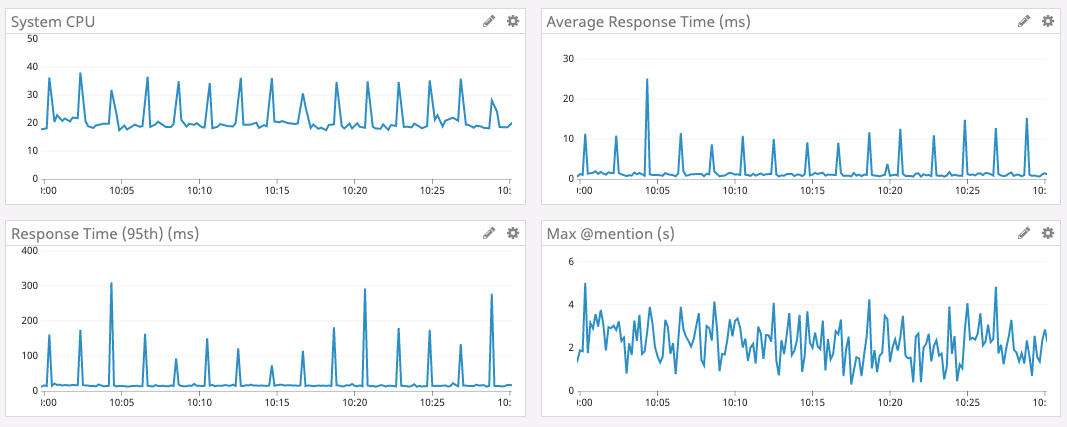
\includegraphics[width=\textwidth]{images/golang-gc.png}
\end{center}

Go garbage collector does its work and it adds a big latency spike.


\end{frame}


\begin{frame}
\frametitle{Real-World Example: Discord}

Rust version performed better than the Go version on latency, CPU, and memory usage.

See the following graphs that compare Rust (blue) to Go (purple): 
\begin{center}
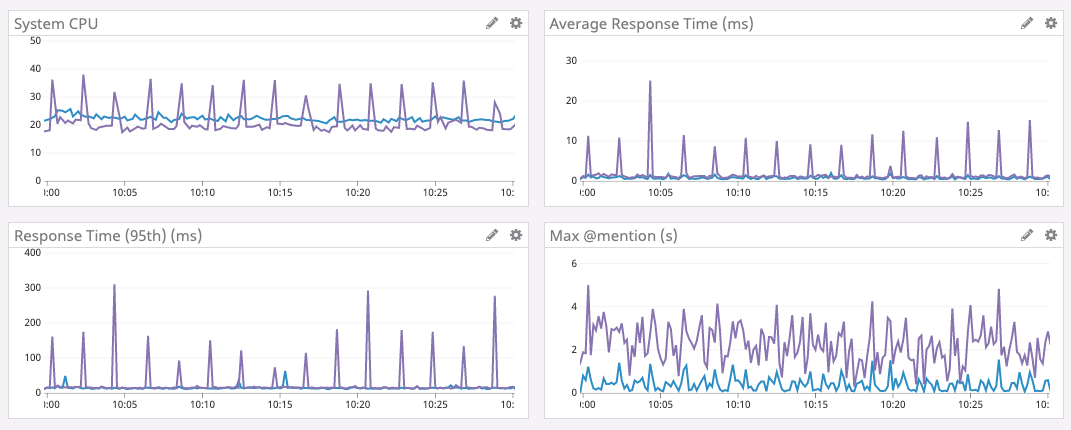
\includegraphics[width=\textwidth]{images/rust-vs-go.png}
\end{center}

\end{frame}


\begin{frame}
\frametitle{Rules}

We talked about the why of ownership, but not the what.

\begin{enumerate}
	\item Every value has a variable that is its owner.
	\item There can be only one owner at a time.
	\item When the owner goes out of scope, the value is dropped.
\end{enumerate}

Note a distinction between the value itself and the variable that owns it.\\
\quad \texttt{let x = 42;}

\end{frame}


\begin{frame}[fragile]
\frametitle{Out of Scope}

Variable scope rules look like scope rules in other C-like languages.

They are rigidly enforced by the compiler.

\begin{lstlisting}[language=Rust]
  fn foo() {
    println!("start");
    { // s does not exist
      let s = "Hello World!";
      println!("{}", s);
    } // s goes out of scope and is dropped
  }
\end{lstlisting}


\begin{center}
	
\includegraphics[width=0.4\textwidth]{images/i-let-him-go.jpg}
\end{center}

\end{frame}


\begin{frame}[fragile]
\frametitle{Stack and Heap}

The same principle applies in terms of heap allocated memory.


\begin{lstlisting}[language=Rust]
  fn main() {
    let s1 = String::from("hello");
    println!("s1 = {}", s1);
  }
\end{lstlisting}

A string has a stack part (left) and a heap part (right) that look like:
\begin{center}
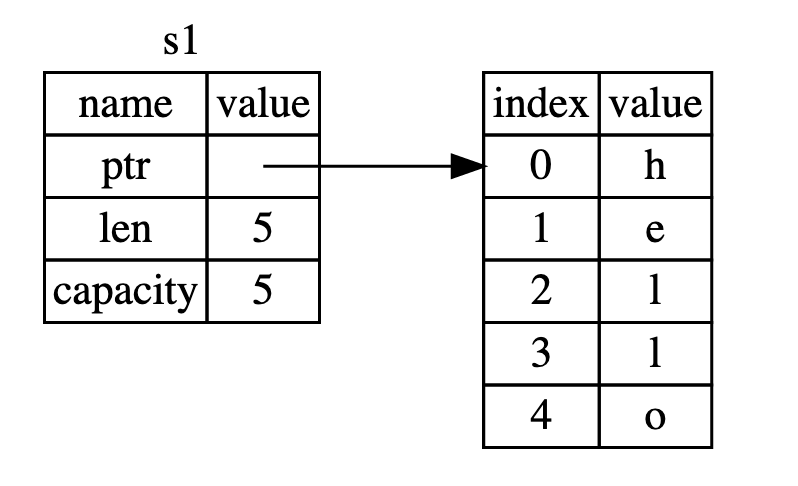
\includegraphics[width=0.5\textwidth]{images/string.png} 
\end{center}

\end{frame}


\begin{frame}
\frametitle{Back to Rule 2}

That covers rules one and three.

But that second rule is interesting, because of the ``at a time'' at the end: it means that there exists the concept of transfer of ownership.


\end{frame}

\begin{frame}[fragile]
\frametitle{What's yours is mine}

Move semantics have to do with transferring ownership from one variable to another.

Some types use copy semantics instead, such as simple types.

Copy semantics are great when copies are cheap and moving would be cumbersome. 

\begin{lstlisting}[language=Rust]
  fn main() {
   	let x = 5;
	let y = x;
  }
\end{lstlisting}


\end{frame}

\begin{frame}[fragile]
\frametitle{Move instead}

But simple types are the exception and not the rule. Let's look at what happens with types with a heap component:

\begin{lstlisting}[language=Rust]
  fn main() {
    let s1 = String::from("hello");
    let s2 = s1;
  }
\end{lstlisting}


Rust won't automatically create a copy if you don't ask explicitly. 

(You ask explicitly by calling \texttt{clone()}).

\end{frame}


\begin{frame}
\frametitle{Move instead}

Here's what actually happens:

\begin{center}
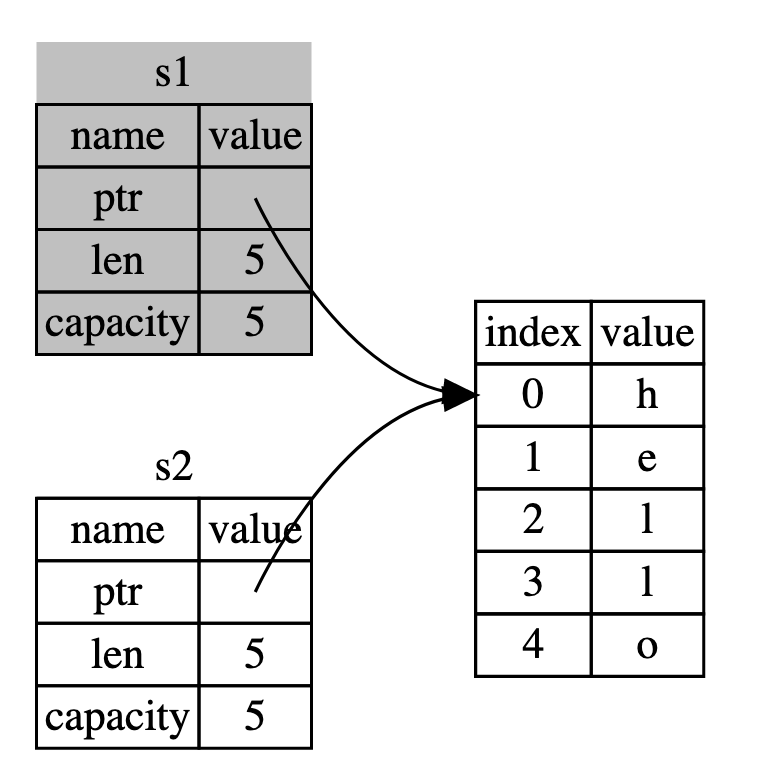
\includegraphics[width=0.35\textwidth]{images/string-rust.png}
\end{center}

If both \texttt{s1} and \texttt{s2} were pointing to the same heap memory, it would violate the second rule of ownership!

\begin{center}
	
\includegraphics[width=0.35\textwidth]{images/highlander.jpeg}
\end{center}

\end{frame}


\begin{frame}[fragile]
\frametitle{Not Allowed}

An attempt to use \texttt{s1} will result in a compile-time error.

\begin{lstlisting}[language=Rust]
  fn main() {
    let x = 5;
    let y = x;
    dbg!(x, y); // Works as you would expect!

    let x = Vec<u32>::new(); // similar to the std::vector type in C++
    let y = x;
    dbg!(x, y); // x has been moved, this is a compiler error!
  }
\end{lstlisting}

\end{frame}


\begin{frame}[fragile]
\frametitle{This is Helpful}

The compiler is even kind enough to tell you what went wrong and why:

{\scriptsize
\begin{verbatim}
plam@amqui ~/c/p/l/l/L02> cargo run
   Compiling move v0.1.0 (/home/plam/courses/p4p/lectures/live-coding/L02)
error[E0382]: use of moved value: `x`
 --> src/main.rs:8:10
  |
6 |     let x = Vec::<u32>::new(); // similar to the std::vector type in C++
  |         - move occurs because `x` has type `std::vec::Vec<u32>`, which does 
              not implement the `Copy` trait
7 |     let y = x;
  |             - value moved here
8 |     dbg!(x, y); // x has been moved, this is a compiler error!
  |          ^ value used here after move

error: aborting due to previous error

For more information about this error, try `rustc --explain E0382`.
error: could not compile `move`.

To learn more, run the command again with --verbose.
\end{verbatim}
}
\end{frame}


\begin{frame}[fragile]
\frametitle{It's Dangerous to Go Alone, Take This}

Move semantics also make sense when returning a value from a function.

\begin{lstlisting}[language=Rust]
  fn make_string() -> String {
    let s = String::from("hello");
    return s;
  }

  fn main() {
    let s1 = make_string();
    println!("{}", s1);
  }
\end{lstlisting}

\end{frame}


\begin{frame}[fragile]
\frametitle{Wait, come back with that...}

This works in the other direction, too: passing a variable as an argument to a function results in either a move or a copy (depending on the type).

You can have them back when you're done only if the function in question explicitly returns it! 


\begin{lstlisting}[language=Rust]
  fn main() {
    let s1 = String::from("world");
	use_string( s1 ); // Transfers ownership to the function being called
	// Can't use s1 anymore!
  }
  
fn use_string(s: String) {
    println!("{}", s); 
    // String is no longer in scope - dropped
}
\end{lstlisting}

This one is easy to fix... clone or return all the thing?

Maybe we can let a function borrow it...

\end{frame}


\begin{frame}
\frametitle{But Do the Rules Work?}

Consider this from the perspective of things that can go wrong in a C program.

\begin{itemize}
	\item Memory leak (fail to deallocate memory)
	\item Double-free
	\item Use-after-free
	\item Accessing uninitialized memory
	\item Stack values going out of scope when a function ends
\end{itemize}

(We'll eventually learn to break rules in a future lecture)

\end{frame}


\begin{frame}
\frametitle{A free lunch?}

 Rust of course doesn't solve every problem in the world. 
 
It does solve memory management well. 

I wouldn't even say that it requires more of the programmer: it requires more of the programmer at compile-time, not at debug-time.

Downsides: 

\begin{itemize}
	\item Static typing
	\item Ecosystem
	\item Compiler
\end{itemize}


\end{frame}



\end{document}

